\section{Ημερολόγιο}

Μία αναμενόμενη απαίτηση της υλοποίησης είναι η διατήρηση των μετρήσεων για την
μετέπειτα ανάκτηση και επεξεργασία τους με σκοπό την εξαγωγή συμπερασμάτων ή τη
λήψη αποφάσεων για την κατάσταση του μέσου. Το Ημερολόγιο μετρήσεων αναλαμβάνει
τη διαχείριση εγγραφών που παρέχουν αυτήν την πληροφορία.

%
% LogRecord
%

\subsection{Δομή εγγραφής}

Σημείο κεντρικού ενδιαφέροντος του Ημερολογίου είναι οι εγγραφές.
Καθότι ανήκει σε ημερολόγιο, κάθε εγγραφή είναι άρρηκτα συνδεδεμένη με μία
ημερομηνία\slash ώρα (εφεξής αναφερόμενη απλά ως «ημερομηνία»), που προσδιορίζει
τη χρονική τοποθέτησή της και χρησιμεύει ως κριτήριο αναζήτησης -- το μοναδικό
που υποστηρίζεται από το Ημερολόγιο σε αυτήν την υλοποίηση.
Εκτός από την ημερομηνία, τηρούνται και τα στοιχεία της μέτρησης, όπως οι
συντεταγμένες όπου έγινε η δειγματοληψία και, σαφώς, οι ενδείξεις των
αισθητήριων οργάνων. Το σχήμα \ref{fig:log:record} παρουσιάζει τη δομή κάθε
εγγραφής.

\begin{figure}
    \caption{Δομή μίας εγγραφής Ημερολογίου.\label{fig:log:record}}
    \begin{center}\begin{tabu} spread 0pt {|X|X|X|X|X|X|X|X|X|X|X|}


    \multicolumn6{c}{
        $\overbrace{\rule{4cm}{0pt}}^{\text{ημερομηνία}}$}              &
    \multicolumn5{c}{
        $\overbrace{\rule{3.2cm}{0pt}}^{\text{στοιχεία μέτρησης}}$}     \\

    \hline\rowfont[c]{}
    \verb~YY~           &
    \verb~ΜΜ~           &
    \verb~DD~           &
    \verb~HH~           &
    \verb~mm~           &
    \verb~ss~           &
    \verb~X~            &
    \verb~Y~            &
    \verb~Τ~            &
    \verb~RH~           &
    \verb~pH~           \\
    \hline

    \end{tabu}\end{center}
\end{figure}

Είναι φανερό ότι η ημερομηνία καταλαμβάνει ένα πολύ μεγάλο μέρος της εγγραφής
και ο λόγος είναι ότι αναπαριστάται σε BCD. Ο συμβολισμός BCD (Binary-Coded
Decimal notation -- Δυαδικά Κωδικοποιημένος Δεκαδικός συμβολισμός), όπως
χρησιμοποιείται στην προκειμένη, απαιτεί ένα Byte για την αναπαράσταση
οποιουδήποτε αριθμού του δεκαδικού συστήματος αρίθμησης από 0 μέχρι 99· εύρος
ικανό να καλύψει τις ανάγκες του Ημερολογίου.

Κύριος λόγος για την επιλογή του συμβολισμού BCD για την ημερομηνία είναι η
αμεσότητα μετατροπής της από αριθμό σε κείμενο, και αντιστρόφως. Πρακτικά, αυτό
σημαίνει ότι είναι ταχύτερη η μετατροπή της κάθε εγγραφής και, κατ' επέκταση
μίας πληθώρας εγγραφών, σε κείμενο που προορίζεται για εμφάνιση σε χρήστη.
% Παράδειγμα ή αναφορά σε BCDDate.

Το μειονέκτημα είναι ότι δεσμεύεται πολύ περισσότερος χώρος από ότι ουσιαστικά
αξιοποιείται. Για παράδειγμα, το ίδιο εύρος ημερομηνιών θα μπορούσε να καλυφθεί
από έναν αριθμό 32-bit που διατηρεί το πλήθος δευτερολέπτων που έχουν παρέλθει
από την ημερομηνία αναφοράς (την παλαιότερη υποστηριζόμενη ημερομηνία). Ωστόσο,
αυτή η προσέγγιση θα απαιτούσε την αναγωγή των συνιστωσών της ημερομηνίας (έτος,
μήνας, μέρα \etc.) κάθε φορά που χρειαζόταν μία εξ αυτών.

%Από την πλευρά του ημερολογίου, κάθε εγγραφή φέρει, υποχρεωτικά, την ημερομηνία
%και ώρα της. Βάσει αυτής

%Το Ημερολόγιο υλοποιείται θεωρώντας ότι η ημερομηνία κάθε εγγραφής είναι
%μοναδική. Επίσης, η ημερομηνία τίθεται από

\subsubsection{Δομή ημερομηνίας}

Οι συνιστώσες της ημερομηνίας (σχήμα \ref{fig:log:record}), αποτελούν μέλη της
δομής \verb~BCDDate~. Η δομή αυτή έχει οριστεί για την κάλυψη των αναγκών του
Ημερολογίου στην αποθήκευση και αναζήτηση εγγραφών καθώς και για την παροχή ενός
κοινού τρόπου ανταλλαγής ημερομηνιών μεταξύ των δομικών στοιχείων της
υλοποίησης. Ο ορισμός της είναι ο ακόλουθος:
\begin{lstlisting}
typedef struct {
    uint8_t year;
    uint8_t mon;
    uint8_t date;
    uint8_t hour;
    uint8_t min;
    uint8_t sec;
} BCDDate;
\end{lstlisting}

Τα μέλη της έχουν οριστεί σε φθίνουσα σειρά σπουδαιότητας με τρόπο που
διευκολύνεται η σύγκριση μεταξύ ημερομηνιών αυτής της δομής. Αρχικά συγκρίνεται
το πρώτο -- πλέον σημαντικό -- Byte κάθε ημερομηνίας, δηλαδή τα έτη. Εφόσον
είναι ίσα, ακολουθεί σύγκριση με το αμέσως επόμενο, σε σπουδαιότητα, Byte, αυτό
του μήνα, και η διαδικασία συνεχίζεται για όλα τα Byte ή έως ότου εντοπιστεί
κάποια διαφοροποίηση, η οποία κρίνει και το ποια ημερομηνία είναι μεγαλύτερη.
Η διαδικασία σύγκρισης που ακολουθείται είναι ίδια με αυτήν μεταξύ δύο μη
προσημασμένων αριθμών μεγάλου μήκους.

%
% LogRecordSet
%

\subsection{Ομάδα εγγραφών}
Τυπικά, δοθέντων δύο ημερομηνιών, το Ημερολόγιο είναι σε θέση να επιστρέψει όλες
τις ενδιάμεσες εγγραφές. Ωστόσο, η άμεση και μαζική επιστροφή τους είναι
απαγορευτική λόγω των περιορισμένων πόρων του μικροελεγκτή καθώς απαιτείται
δέσμευση χώρου στην κύρια μνήμη, δυνητικά, για όλες τις εγγραφές του
Ημερολογίου.
%
%Επιπλέον, απαιτείται
%η προσπέλαση του υποκείμενου αποθηκευτικού μέσου για την ανάκτηση εγγραφών εκ
%των οποίων μόλις ένα μικρό μέρος μπορεί να έχει ενδιαφέρον στην εκάστοτε
%περίπτωση. Για παράδειγμα, παρότι έχουν δοθεί δύο ημερομηνίες που καλύπτουν όλο
%το εύρος των εγγραφών, μπορεί να πρέπει να επιστραφούν σε μία εξωτερική οντότητα
%μόνο οι πρώτες δέκα, καθώς τα αποτελέσματα έχουν ζητηθεί να επιστραφούν
%σελιδοποιημένα. Είναι σαφές πως μία τέτοια τακτική μειώνει σημαντικά την απόδοση
%του συστήματος.

Αντιθέτως, η προσπέλαση των εγγραφών πραγματοποιείται σε βήματα. Αρχικά,
εκτελείται αναζήτηση βάσει των επιθυμητών ημερομηνιών από όπου επιστρέφεται το
πλήθος των εγγραφών που εντοπίστηκαν, καθώς και μία δομή \verb~LogRecordSet~. H
δομή αυτή αναπαριστά το σύνολο (ή ομάδα) των εντοπισμένων εγγραφών.
Ωστόσο, στην πραγματικότητα, περιέχει μόνο την πληροφορία που επιτρέπει να
εξαχθεί η επόμενη εγγραφή.
Για την οποιαδήποτε επενέργεια στις πραγματικές εγγραφές, παρέχονται ξεχωριστές
συναρτήσεις, κάθε μία δεχόμενη τη δομή \verb~LogRecordSet~. Με τον τρόπο αυτό
γίνεται γνωστή η κατάσταση του τρέχοντος συνόλου ώστε να προσαρμόζεται
καταλλήλως η συμπεριφορά της εκάστοτε συνάρτησης, ενώ δίνεται η δυνατότητα
ενημέρωσης της δομής μετά την ολοκλήρωση των εργασιών.

%Για τις τρέχουσες απαιτήσεις της υλοποίησης, η δομή \verb~LogRecordSet~ ορίζεται
%ως ακολούθως:
%\begin{flushleft}
%\begin{verbatim}
%typedef struct {
%    uint8_t index;
%    uint8_t count;
%} LogRecordSet;
%\end{verbatim}
%\end{flushleft}

%Το μέλος \verb~index~ αναπαριστά τη θέση. \verb~count~

\subsection{Οργάνωση εγγραφών}

Στο σημείο αυτό αναλύεται πώς διαχειρίζεται το Ημερολόγιο τον αφιερωμένο
αποθηκευτικό χώρο για τις εγγραφές του. Παρότι περιγράφονται δύο σχεδιασμοί,
ωστόσο, αποτελούν όψεις του ίδιου νομίσματος· και οι δύο υλοποιούνται σε κώδικα
και λειτουργούν ο ένας πάνω από τον άλλο, προσδίδοντας διαφορετικά επίπεδα
αφαίρεσης. Στο πρώτο κομμάτι περιγράφεται  ενώ στο δεύτερο, πώς υλοποιείται η
διαχείριση των εγγραφών σε φυσικό επίπεδο.

\subsubsection{Επίπεδο κυλιόμενου πίνακα}
Σε υψηλό αφαιρετικό επίπεδο, ο αποθηκευτικός χώρος νοείται ως ένας μονοδιάστατος
πίνακας, εκτεταμένος σε διαδοχικές θέσεις μνήμης, κάθε στοιχείο του οποίου είναι
μία εγγραφή. Οι εγγραφές τοποθετούνται σε αύξουσα σειρά βάσει της ημερομηνίας
τους, με την παλαιότερη να βρίσκεται πάντα στην πρώτη θέση του πίνακα.

Υπό φυσιολογικές συνθήκες, κάθε νέα εγγραφή διαθέτει ημερομηνία μεγαλύτερη των
υπαρχόντων και, συνεπώς, προστίθεται μετά την τρέχουσα τελευταία εγγραφή.
Ωστόσο, η τροποποίηση των ρυθμίσεων της συσκευής -- για την ακρίβεια της
ημερομηνίας\slash ώρας --  είναι πιθανό να προκαλέσει την παραγωγή νέων εγγραφών
με ημερομηνία που προηγείται ορισμένων αποθηκευμένων εγγραφών. Η νέα εγγραφή
διατηρείται πάντα, σύμφωνα με την πεποίθηση ότι οι νέες ρυθμίσεις που προκαλούν
αυτήν τη χρονική ασυνέχεια, έχουν γίνει με σκοπό τη διόρθωση μίας εσφαλμένης
κατάστασης της συσκευής. Το ερώτημα τίθεται για τις παλαιότερα αποθηκευμένες
εγγραφές που διαθέτουν, πλέον, νεότερη ημερομηνία σε σχέση με κάποια νέα
εγγραφή.

Εάν διατηρούνται, τότε μετρήσεις που έχουν γίνει σε παρελθοντικό χρόνο
αναμιγνύονται με τις νέες μετρήσεις, ενδεχομένως, νοθεύοντας τα αποτελέσματά
τους, εφόσον υπάρχουν αποκλίσεις μεταξύ παλαιών και νέων. Για την αποφυγή
τέτοιων αβεβαιοτήτων, το Ημερολόγιο απορρίπτει τις προϋπάρχουσες εγγραφές, η
ημερομηνία των οποίων έπεται κάποιας νέας, προς αποθήκευση, εγγραφής.

Οι επιλογές που έχουν περιγραφεί μέχρι στιγμής, καθιστούν δυνατή την προσπέλαση
υπαρχόντων και την εισαγωγή νέων εγγραφών σε σταθερό χρόνο, ενώ επιτρέπουν την
εύρεση εγγραφών βάσει ημερομηνίας σε χρόνο $O(\log n)$ (μέσω δυαδικής
αναζήτησης). Και τα δύο είναι χαρακτηριστικά που εγγυούνται μειωμένο πλήθος
προσβάσεων στη συσκευή μόνιμης αποθήκευσης, η οποία, κατά πάσα πιθανότητα,
χαρακτηρίζεται από υψηλότερους χρόνους προσπέλασης. Ένα δεύτερο πλεονέκτημα
είναι η κατά το μέγιστο αξιοποίηση του αφιερωμένου αποθηκευτικού χώρου καθώς
αποθηκεύονται μόνο πραγματικά δεδομένα και όχι δευτερεύοντα βοηθητικά (όπως, για
παράδειγμα, δείκτες επόμενου στοιχείου στην περίπτωση χρήσης συνδεδεμένης
λίστας).
Βέβαια, όλα αυτά είναι άμεση απόρροια της
έλλειψης ανάγκης για ενημέρωση και διαγραφή εγγραφών.

Ένα τελευταίο χαρακτηριστικό του Ημερολογίου είναι η αντιμετώπιση της εξάντλησης
του διαθέσιμου αποθηκευτικού χώρου. Σε αυτήν την περίπτωση, επιλέγεται η
απόρριψη της παλαιότερης εγγραφής με την (νοητή) μετακίνηση του πίνακα κατά μία
θέση ώστε να δημιουργηθεί μία νέα θέση στο τέλος του (εξού και ο χαρακτηρισμός
ως «κυλιόμενος»). Σαφώς, ο αντίστοιχος μηχανισμός αναλαμβάνεται από χαμηλότερο
επίπεδο της υλοποίησης. Ωστόσο, αξίζει να σημειωθεί ότι στο μεγαλύτερο κομμάτι
της υλοποίησης ο αποθηκευτικός χώρος αντιμετωπίζεται με αυτόν τον τρόπο· ως ένας
πίνακας όπου το πρώτο του στοιχείο είναι η παλαιότερη εγγραφή, το πραγματικό
περιεχόμενο της οποίας αλλάζει ανά πάσα στιγμή, και ότι οι εγγραφές εκτείνονται
σε αύξουσα σειρά και καλύπτουν μερικώς ή πλήρως τις θέσεις του πίνακα.

\subsubsection{Επίπεδο κυκλικής ουράς}

Επειδή κύριας σημασίας είναι η διατήρηση των τελευταίων μετρήσεων, σε περίπτωση
εξάντλησης του διαθέσιμου αποθηκευτικού χώρου, οι νέες εγγραφές αντικαθιστούν
τις παλαιότερες. Η συμπεριφορά αυτή μπορεί να αποδοθεί από μία απλουστευμένη
μορφή δακτυλίου (ή κυκλικής ουράς), όπου επιτρέπεται μόνο η εισαγωγή στοιχείων
στη δομή με υποστήριξη επικάλυψης των παλαιοτέρων. Βέβαια στην πραγματικότητα, ο
χώρος αποθήκευσης είναι ένας πίνακας από διαδοχικά Byte ή, λίγο πιο αφαιρετικά,
από διαδοχικές θέσεις μεγέθους \verb~LogRecord~. Προκειμένου να υλοποιηθεί η
συμπεριφορά του δακτυλίου, απαιτείται η τήρηση ενός δείκτη που προσδιορίζει τη
θέση του πρώτου στοιχείου καθώς και ενός δεύτερου δείκτη για την τελευταία
\parencite[131]{kolias04}. Ωστόσο, αντί για δείκτη τέλους, τηρείται το πλήθος
των διαθέσιμων εγγραφών. Αυτό έχει το πλεονέκτημα ότι είναι άμεσα γνωστό το
πλήθος των εγγραφών χωρίς να απαιτούνται αλγεβρικές πράξεις για την εξαγωγή του
και, κυρίως, διευκολύνει την αναγνώριση ενός πλήρως γεμάτου από έναν πλήρως
άδειο δακτύλιο (περιπτώσεις κατά τις οποίες οι δείκτες αρχής και τέλους έχουν
την ίδια τιμή).

Στο σχήμα \ref{fig:log:structure} παρουσιάζεται πώς αντιστοιχίζονται
αμφιμονοσήμαντα τα στοιχεία του ιδεατού κυλιόμενου πίνακα
(\ref{fig:log:structure}α) με τα στοιχεία όπως αυτά είναι πραγματικά
αποθηκευμένα στην κυκλική ουρά (\ref{fig:log:structure}β). Σημειώνεται το
εμφανές, ότι για την αναγωγή από το ένα στοιχείο στο άλλο απαιτείται σταθερός
χρόνος.

\begin{figure}
    \caption{Λογικά επίπεδα δομής αποθήκευσης.\label{fig:log:structure}}
    \begin{center}%
    \def\svgwidth{0.7\textwidth}
    \input{img/log_structure.pdf_tex}
    \end{center}
\end{figure}


\section{Ανάθεση εργασιών}

% \nref : Drivesystem chapter
Στο κεφάλαιο του υποσυστήματος κίνησης
παρουσιάζεται ο υποκείμενος μηχανισμός για τον έλεγχο της κίνησης της κεφαλής
της συσκευής. Συγκριτικά .. αυτό που επιτυγχάνει είναι η 


Ωστόσο, στο πλαίσιο της υλοποίησης, η χρήση του υποσυστήματος κίνησης είναι
άρρηκτα συνδεδεμένη με την πραγματοποίηση μέτρησης· η κεφαλή μετακινείται σε μία
θέση με σκοπό τη δειγματοληψία και καταχώρηση της μέτρησης των αισθητήρων για
εκείνο το σημείο του υλικού. Αυτή η πρόσθετη λειτουργία παρέχεται από τη μονάδα
εργασίας (\te{task}).


\subsubsection{Δειγματοληψία σε νέα θέση}

Όπως αναφέρεται, % \nref : Μέγιστη κοινή μετατόπιση
η μετακίνηση της κεφαλής πραγματοποιείται σε στάδια. Επομένως, στην απλή της
μορφή, μία εργασία περιλαμβάνει τα ακόλουθα στάδια:
\begin{enumerate}
    \item Μετατόπιση σε ένα νέο ζεύγος συντεταγμένων XY.
    \item Διείσδυση της κεφαλής στο παρακολουθούμενο μέσο.
    \item Λήψη μέτρησης των αισθητήρων και καταχώρησή τους στο Ημερολόγιο
    (σ.~\pageref{sec:log}).
    \item Ανύψωση της κεφαλής.
\end{enumerate}

Δεδομένου ότι η κεφαλή βρίσκεται ανυψωμένη (προεπιλεγμένη θέση κατόπιν
παλιννόστησης), % \nref : Παλιννόστηση
τα δύο πρώτα στάδια πραγματοποιούνται αυτομάτα από τον
υποκείμενο μηχανισμό. Κατά την ολοκλήρωση της μετακίνησης της κεφαλής
(συμπεριλαμβανομένης και της διείσδυσής στο μέσο), το υποσύστημα κίνησης
ενημερώνει για το συμβάν (μέσω επανάκλησης) το υποσύστημα εργασίας (ή όποιο άλλο
του έχει δηλωθεί).

Στο σημείο αυτό, η υπομονάδα εργασίας εκτελεί το 3\tsup{ο} στάδιο. Κατόπιν,
προκαλεί την ανύψωση της κεφαλής, η οποία εκτελείται ασύγχρονα (όπως συμβαίνει,
άλλωστε, με κάθε κίνηση της κεφαλής). Το υποσύστημα εργασίας ειδοποιείται ξανά
όταν η κεφαλή έχει επανατοποθετηθεί στην κορυφαία της θέση. Πλέον, εφόσον
απαιτείται, είναι δυνατό να δρομολογηθεί μία νέα μέτρηση προκαλώντας τη
μετατόπιση της κεφαλής σε νέες συντεταγμένες XYZ με $\text{Z} = 0$, ώστε το
υποσύστημα εργασίας να ειδοποιηθεί όταν η κεφαλή βρίσκεται σε θέση για νέα
μέτρηση.

Στο σχήμα \ref{fig:task:samples} παρουσιάζεται πώς το υποσύστημα εργασίας
προκαλεί την αρχική ενεργοποίηση τους υποσυστήματος κίνησης (για τη μετακίνηση
σε νέα θέση) και πώς οι διαδοχικές διεκπεραιώσεις της μετακίνησης της κεφαλής
οδηγούν, σταδιακά, στην ολοκλήρωση του ανατεθειμένου πλήθους μετρήσεων.

\begin{figure}
    \caption{
    \label{fig:task:samples}}
%    \includegraphics{}
\end{figure}

Ένα αναγκαίο στοιχείο για την πραγματοποίηση πολλαπλών μετρήσεων είναι η ύπαρξη
ενός μηχανισμού για την παραγωγή νέων, προς δειγματοληψία, θέσεων. Ένας τέτοιος
μηχανισμός θα μπορούσε να λαμβάνει υπόψη προηγούμενες μετρήσεις ώστε να
προτιμώνται τοποθεσίες που έχουν καιρό να υποστούν εξέταση ή εκείνες στις οποίες
είχαν εντοπιστεί κρίσιμες τιμές. Ωστόσο, στο πλαίσιο της υλοποίησης, ο
μηχανισμός αρκείται στην παραγωγή τυχαίων θέσεων που βασίζονται, ελαφρώς, στην
τρέχουσα ημέρα και ώρα της συσκευής
% \nref : RTC
και στην τρέχουσα θέση της κεφαλής.


\subsubsection{Εκτιμώμενος χρόνος ολοκλήρωσης}

Στο σχήμα \ref{fig:task:samples} γίνεται αναφορά σε εκτίμηση του χρόνου
ολοκλήρωσης η οποία εκτελείται όποτε η επανάκληση αναφέρει ότι το υποσύστημα
κίνησης είναι απασχολημένο (\te{BUSY}). Ο λόγος ύπαρξης του μηχανισμού είναι η
παροχή μίας ένδειξης του χρόνου για τον οποίο το υποσύστημα κίνησης, καθώς και
όλες οι λειτουργίες που βασίζονται σε αυτόν, είναι αδύνατο να χρησιμοποιηθούν
έως ότου παρέλθει. Χαρακτηριστική περίπτωση χρήσης του εκτιμώμενου χρόνου είναι
στο πεδίο κεφαλίδας HTTP \te{Retry-After} κατά τις αποκρίσεις με κωδικούς
κατάστασης 202 και 503 (βλ. \nameref{sec:network:impl-resources},
σ.~\pageref{sec:network:impl-resources}).

Όπως αναφέρεται στο Υποσύστημα Κίνησης
(σσ.~\pageref{ssubsec:motor:routing},%
\pageref{ssubsec:motor:common-translation}),
η μετατόπιση της κεφαλής σε νέα θέση πραγματοποιείται σε τρία, το πολύ, στάδια·
κοινή μετατόπιση στο επίπεδο X-Y, υπολειπόμενη μετατόπιση σε άξονα X ή Υ και
μετατόπιση σε άξονα Z. Πριν την εκκίνηση κάθε σταδίου, και ενώ οι κινητήρες
βρίσκονται σε ηρεμία, αναγγέλλεται από το υποσύστημα κίνησης (μέσω της
επανάκλησης) ο νέος προορισμός και η αλλαγή της κατάστασής του σε \te{BUSY}. Η
πληροφορία αυτή σε συνδυασμό το υπολειπόμενο πλήθος μετρήσεων μπορεί να
χρησιμοποιηθεί για τον υπολογισμό της εκτίμησης.

\begin{figure}
    \caption{Ανανέωση 
    \label{fig:task:estimate-update}}
    \begin{center}
    \end{center}
\end{figure}

Το σχήμα \ref{fig:task:estimate-update} παρουσιάζει τις συνιστώσες της εργασίας
καθώς και τις στιγμές που αναγγέλλεται η ολοκλήρωση ενός μέρους της μετατόπισης
(σημεία \te{BUSY}).
Όπως αναφέρεται προηγουμένως, η νέα θέση της κεφαλής στο επίπεδο X-Y
υπολογίζεται τη στιγμή ολοκλήρωσης της προηγούμενης εργασίας. Αυτή η σχεδιαστική
επιλογή καθιστά αδύνατο τον ακριβή υπολογισμό του χρόνου ολοκλήρωσης του συνόλου
των εργασιών καθώς οι θέσεις που, τελικά, θα προκύψουν είναι άγνωστες σε
προγενέστερη στιγμή της εκτέλεσης.

Για το λόγο αυτό χρησιμοποιείται ένας αναμενόμενος χρόνος μετατόπισης της
κεφαλής στο επίπεδο X-Y για τις υπολειπόμενες εργασίες ο οποίος, όσο μεγαλύτερο
το πλήθος εργασιών, τόσο μεγαλύτερη απόκλιση από τον πραγματικό χρόνο που
τελικά θα απαιτηθεί. Ωστόσο, καθώς ολοκληρώνονται τα επιμέρους στάδια κάθε
εργασίας και πραγματοποιείται νέα εκτίμηση (σημεία αναγγελίας \te{BUSY}), ο
εκτιμώμενος χρόνος γίνεται ολοένα πιο έγκυρος. Η απόκλιση της εκτίμησης του
χρόνου ολοκλήρωσης της τελευταίας εργασίας κυμαίνεται στα 2, περίπου,
δευτερόλεπτα, μετρική αποδεκτή για τις απαιτήσεις της υλοποίησης.

Η εκτίμηση του χρόνου ολοκλήρωσης του φόρτου εργασίας καθώς και η ώρα κατά την
οποία πραγματοποιήθηκε η εκτίμηση, διατηρούνται. Όποτε προκύπτει ανάγκη για την
επιστροφή του αναμενόμενου χρόνου ολοκλήρωσης ξεκινώντας κάποια δεδομένη χρονική
στιγμή, αρκεί να αφαιρεθεί από εκείνη την ώρα, η ώρα της τελευταίας εκτίμησης
και να συγκριθεί το αποτέλεσμα με την εκτίμηση χρόνου για να διαπιστωθεί πόσος
εκτιμημένος χρόνος έχει παρέλθει.


\subsubsection{Εκκίνηση εργασίας}
\label{ssubsec:task:initiate}

Η δειγματοληψία του μέσου είναι δυνατό να ξεκινήσει με δύο τρόπους· κατόπιν
προτροπής εξωτερικής οντότητας ή από το ίδιο το σύστημα υπό τις κατάλληλες
συνθήκες. Η εκκίνηση εργασιών από εξωτερική οντότητα περιγράφεται στη μέθοδο
\te{POST} του πόρου μετρήσεων του διακομιστή
(σ.~\pageref{ssubsec:network:measurement-post}) και παρέχεται κυρίως για λόγους
εξακρίβωσης λειτουργίας.

Η κύρια πηγή εκκίνησης των κύκλων εργασιών παραμένει το ίδιο το σύστημα.
Για το σκοπό αυτό, κρίνεται
αρκετή η τήρηση της ώρας της πιο πρόσφατης μέτρησης και μίας ένδειξης για το
ελάχιστο επιθυμητό διάστημα μεταξύ διαδοχικών κύκλων εργασίας. Επίσης,
απαιτείται η ύπαρξη ενός ελέγχου για την εξακρίβωση του χρόνου που έχει παρέλθει
από την πλέον πρόσφατη μέτρηση μέχρι τη στιγμή που πραγματοποιείται ο έλεγχος.

Προφανώς, η ημερομηνία της πλέον πρόσφατης μέτρησης τίθεται κατά την
αρχικοποίηση της συσκευής (\te{power-on}) βάσει της τελευταίας καταχωρημένης
εγγραφής του ημερολογίου και ενημερώνεται με κάθε νέα πραγματοποιηθείσα μέτρηση.

Ωστόσο, στην πραγματικότητα, ο μηχανισμός βασίζεται στη χρήση χρονοσφραγίδων που
αντιπροσωπεύουν τα λεπτά που έχουν παρέλθει από την αρχή της ημέρας για κάθε
ημερομηνία. Για την ακρίβεια, επιλέγεται η ημέρα να χωρίζεται σε 240 κβάντα, ενώ
κάθε χρονοσφραγίδα προσδιορίζει κάποια στιγμή της ημέρας ως ένα πλήθος τέτοιων
κβάντων. Όποτε προκύπτει ανάγκη για τον έλεγχο του χρονικού διαστήματος που έχει
παρέλθει μεταξύ πρόσφατης και τρέχουσας ώρας, η τρέχουσα ώρα ανάγεται σε
χρονοσφραγίδα (δηλαδή, σε κβάντα των 6 λεπτών) και συγκρίνεται με τη
χρονοσφραγίδα της μέτρησης (σχήμα \ref{fig:task:interval}).

\begin{figure}
    \caption{Αντιστοίχηση ωρών σε κβάντα και υπολογισμός χρονικού διαστήματος.
    \label{fig:task:interval}}
    Με n συμβολίζεται η κάθε ώρα της ημέρας και κυμαίνεται μεταξύ 0 και 23, ενώ
    για κάθε ώρα ορίζονται 10 κβάντα. Συνολικά, μία μέρα διαθέτει 240 κβάντα.
    \begin{center}
    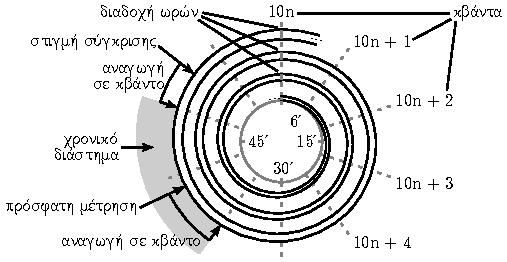
\includegraphics{task_interval}
    \end{center}
\end{figure}

Ο υπολογισμός της χρονοσφραγίδας είναι απλός· οι ώρες μετατρέπονται σε λεπτά και
χωρίζονται σε κβάντα, κατόπιν, προστίθεται η αξία (ευκλείδεια διαίρεση) των
λεπτών σε κβάντα, ως εξής:
\begin{equation}
Q = \frac{60 hrs + min}{q}
\end{equation}
, όπου $q$ η αξία κάθε κβάντου σε λεπτά ($q = 6$).

Ως άμεσο αποτέλεσμα, είναι δυνατή η διάκριση των ωρών με ακρίβεια το πολύ 6
λεπτών. Επιπλέον, η τήρηση μέχρι 240 κβάντων (δηλαδή, μίας ημέρας) συνεπάγεται
ότι οι δύο ημερομηνίες συγκρίνονται μόνο ως προς τις ώρες και τα λεπτά,
αγνοώντας τη διαφορά τους σε ημέρες, μήνες και έτη. Τυπικά, το πρόβλημα αυτό
είναι αμελητέο καθώς η σύγκριση των χρονοσφραγίδων πραγματοποιείται κάθε λίγα
δευτερόλεπτα. Μόνο στην περίπτωση παρατεταμένης διακοπής της τροφοδοσίας του
ρεύματος ενδέχεται να εμφανιστεί κάποια ασυνέχεια με τη μορφή καθυστερημένης
εκκίνησης του επόμενου κύκλου εργασίας που οφείλεται στο ότι η συσκευή αναμένει
να παρέλθει το καθορισμένο πλήθος κβάντων από την τελευταία \emph{ώρα} μέτρησης,
ανεξαρτήτως της ημέρας κατά την οποία πραγματοποιήθηκε.


\subsubsection{Περιοδικός έλεγχος}

Είναι σαφές ότι ο έλεγχος της χρονοσφραγίδας απαιτεί ένα έναυσμα που να προκαλεί
την εκτέλεσή του. Επίσης, θα πρέπει να είναι ικανό να αφυπνίζει τη μονάδα
επεξεργασίας από λειτουργία χαμηλής κατανάλωσης που αυτή τίθεται όσο αναμένει
κάποια νέα εργασία. Σύμφωνα με το εγχειρίδιο της \textcite[38]{atmel13}, ο
χρονομετρητής WDT (\te{Watchdog Timer}) μπορεί να χρησιμοποιηθεί για την
αφύπνιση της MCU από οποιαδήποτε λειτουργία χαμηλής κατανάλωσης.

Ο χρονομετρητής WDT χρησιμοποιεί παλμούς ανεξάρτητου ταλαντωτή και ρυθμίζεται
για περιοδική ενεργοποίηση (μέσα από ένα εύρος πιθανών περιόδων) κατά την οποία
προκαλεί διακοπή ή ακόμα και επανεκκίνηση του μικροελεγκτή (\te{reset})
\parencite[50]{atmel13}. Το δεύτερο είναι ιδιαίτερα σημαντικό για την αποφυγή
ατερμόνων βρόχων αλλά απαιτεί την, από λογισμικού, επανέναρξη του μετρητή πριν
την πρόκληση της επανεκκίνησης \parencite[50]{atmel13}.

Στο πλαίσιο της υλοποίησης, ο WDT ρυθμίζεται μόνο για την αναγγελία διακοπής, η
οποία είτε αφυπνίζει την MCU και εκτελεί τη ρουτίνα εξυπηρέτησης της, είτε
αναμένει την ολοκλήρωση κάποιας άλλης ρουτίνας (για παράδειγμα, την απόκριση σε
κάποιο εισερχόμενο αίτημα HTTP) πριν εκτελεστεί η ίδια για την εκκίνηση του
επόμενου κύκλου εργασίας, εφόσον απαιτείται. Σημειώνεται ότι ο επιλεγμένος
μικροελεγκτής (ATmega328P), υποστηρίζει περιόδους από 16ms μέχρι 8s
\parencite[55]{atmel13}.
